\documentclass[12pt,letterpaper]{article}

\usepackage{graphicx,textcomp}
\usepackage{setspace}
\usepackage{fullpage}
\usepackage{color}
\usepackage[reqno]{amsmath}
\usepackage{amsthm}
\usepackage{fancyvrb}
\usepackage{amssymb,enumerate}
\usepackage[all]{xy}
\usepackage{endnotes}
\usepackage{lscape}
\newtheorem{com}{Comment}
\usepackage{float}
\newtheorem{lem} {Lemma}
\newtheorem{prop}{Proposition}
\newtheorem{thm}{Theorem}
\newtheorem{defn}{Definition}
\newtheorem{cor}{Corollary}
\newtheorem{obs}{Observation}

\usepackage[compact]{titlesec}
\usepackage{dcolumn}
\usepackage{tikz}
\usetikzlibrary{arrows}
\usepackage{multirow}
\usepackage{xcolor}
\newcolumntype{.}{D{.}{.}{-1}}
\newcolumntype{d}[1]{D{.}{.}{#1}}
\definecolor{light-gray}{gray}{0.65}
\usepackage{url}
\usepackage{listings}
\usepackage{color}
\usepackage{adjustbox}
\usepackage{caption}
\captionsetup{justification=centering}

\usepackage{hyperref}

%%%% BIBLIOGRAPHY SETTINGS %%%%

\usepackage[backend=biber, notes, isbn=false, doi=false, url=false]{biblatex-chicago}
\addbibresource{/Users/sarabcidf/Desktop/ASDS/Dissertation/Latex/PopulismBiblio.bib}

\definecolor{codegreen}{rgb}{0,0.6,0}
\definecolor{codegray}{rgb}{0.5,0.5,0.5}
\definecolor{codepurple}{rgb}{0.58,0,0.82}
\definecolor{backcolour}{rgb}{0.95,0.95,0.92}

\lstdefinestyle{mystyle}{
	backgroundcolor=\color{backcolour},   
	commentstyle=\color{codegreen},
	keywordstyle=\color{magenta},
	numberstyle=\tiny\color{codegray},
	stringstyle=\color{codepurple},
	basicstyle=\footnotesize,
	breakatwhitespace=false,         
	breaklines=true,                 
	captionpos=b,                    
	keepspaces=true,                 
	numbers=left,                    
	numbersep=5pt,                  
	showspaces=false,                
	showstringspaces=false,
	showtabs=false,                  
	tabsize=2
}

% Tables %

\usepackage{multirow}
\usepackage{cellspace} % for cell margins
\setlength\cellspacetoplimit{5pt} % Adjust the top margin
\setlength\cellspacebottomlimit{5pt} % Adjust the bottom margin

%%%% SECTIONS FORMATTING %%%%

\titleformat{\section}[hang]
{\normalfont\Large\bfseries}{\thesection}{1em}{}
\titlespacing*{\section}
{0pt}{0pt plus 4pt minus 2pt}{0pt plus 2pt minus 2pt}
\newcommand{\sectionbreak}{\clearpage}

\lstset{style=mystyle}
\newcommand{\Sref}[1]{Section~\ref{#1}}
\newtheorem{hyp}{Hypothesis}

%%%% COVER PAGE %%%%

\title{
	Rethinking Populism: A Computational Approach to Study Populist Rhetoric\\
	\large Dissertation Draft  
}
\author{
	Sara Cid\\  
	Supervisor: Dr. Tom Paskhalis  
}
\date{\today}

%%%% DOCUMENT %%%%

\begin{document}
	
\maketitle

\section*{Abstract}

\noindent This paper introduces a novel computational approach to measure populism, addressing the challenges faced by traditional methods to study populist rhetoric. Using over \textcolor{red}{X} party manifestos from \textcolor{red}{X} Spanish-speaking Latin American countries, spanning from 2000 onwards, this study employs quantitative text analysis and machine learning techniques to quantify levels of populism from the manifestos. This method is highly generalizable, scalable, and does not require labor or resource-intensive processes. Moreover, as an application, this paper explores the relationship between populism and anti-elitism in Latin America, the argument being that in this region, the anti-elitism component might not be as salient in populist movements as it has been previously suggested in the literature. 
 
 %%%% CONTENTS HERE %%%%

\tableofcontents
\listoffigures
\listoftables

\section*{Introduction} 

\vspace{.25cm}
One of the largest challenges that remain in the study of populism is measuring it across contexts, accommodating for different countries, parties and leaders. Measuring populism is crucial to study it, and for researchers to understand its intensity, impact, and how it may interact with other political, social and economic variables or its consequences for democracy. 

Moreover, understanding populism across different national contexts is relevant due to this phenomenon's varied manifestations. Populist movements can emerge in any socio-political environment, influenced by diverse factors such as historical legacies, economic conditions, cultural dynamics, and institutional frameworks. Moreover, populism, being ideologically void, is an extremely diverse phenomenon. Measuring it across contexts enables comparative studies, which allow for identifying patterns, similarities, and differences between populisms. 

Traditional approaches have relied on human-coded analysis or dictionary-based methods of automated content analysis, but these methods are generally labor-intensive, costly, unfeasible for non-experts, and lacking in generalizability and content validity. Therefore, there is a need for alternative measurement techniques in the study of populism.  

In addition, most studies of populism have been based in developed countries and, while Latin America has seen a considerable rise in both left-wing and right-wing populist movements in the last years, this region remains understudied, and there is considerable room to evaluate how well the current definitions and conceptions around populism fit the Latin American context 
\footnote{With the exception of Hawkins, who has carried out extensive studies of Latin American populism, especially for the case of Venezuela}. 

As other authors have found in recent years, machine learning offers a promising solution to these challenges \autocite{coccoHowPopulistAre2022} \autocite{daiMeasuringPopulismContext}. Supervised learning techniques, paired with natural language processing, allow for measurements that can capture the traits of populist discourse in a way that is both scalable and adaptable to different contexts. By training algorithms on a wide range of text data, such as party manifestos, speeches, and other political documents, researchers can develop models that are sensitive to the contextualized nature of populist rhetoric, while going beyond the limitations of previous methods.

Thus, this paper offers one such alternative. Working with over 120 party manifestos from 10 Spanish-speaking Latin American countries from the year 2000 on, and with party ratings coming from an expert survey, a Random Forests algorithm is trained to predict the level of populism in a text. The manifestos are broken into individual sentences, and a Bag of Words approach is followed, vectorizing these sentences to serve as the features for the model. For the target variable, a scale measuring parties' level of populism (as deemed by experts) is used.  

After the model is trained, this paper applies it to investigate the saliency of anti-elitism and people-centrism in Latin American populisms. These two have been established as components of populism in the literature, but a revision is worth exploring for non-Western contexts. Thus, a study is carried out where the level of populism assigned to each party is analyzed against the presence of both people-centric and anti-elitist discourse, determining whether higher degrees of populism are associated with more anti-elitism and people-centrism. 

\section*{Literature} 

\vspace{.25cm}
\textbf{Defining Populism}
\vspace{.25cm}

\noindent Accounts of populism as a concept are abundant in the political science literature. Among the most notable works is Cas Mudde's foundational analysis of this phenomenon. According to Mudde, populism can be reduced to five essential characteristics. Crucially, populists are people-centric and anti-elitist. Populist leaders tend to position themselves as ``the voice of the people" and create an opposition against the ``corrupt elite". The elite can include politicians, parties, business leaders, journalists or others that are portrayed as antagonistic to the interests of the common people, while the latter is portrayed as inherently good and honest\autocite{muddePopulistZeitgeist2004}.

Populism can also be distinguished in its opposition to pluralism and elitism. First, populism is contrary to pluralism, as the first tends to promote a singular, homogeneous notion of the people's will, marginalizing diverse voices, while the latter promotes a system that respects and represents varied interests through dialogue and compromise. Populism is also opposed to elitism. Unlike elitism, which supports governance by a select group deemed superior in competence or status, populism advocates for the empowerment of the common people, proposing a shift in power dynamics \autocite{muddePopulismVeryShort2017}.

The view that populism empowers the common people is supported by other authors as well. Some argue that populists appeal to the ideals and symbols that remind people of their collective power and the foundational myths of democratic governance \autocite{canovanTrustPeoplePopulism1999}, while others stress that the articulation that populist leaders do of disparate social demands into a unified and coherent populist rhetoric is fundamentally democratic \autocite{benvenutoPopulistReasonErnesto2012}.

Finally, populism is compatible with both left and right-wing ideologies, as it itself has little ideological content. These other ideologies provide the policy content of populist parties, and as such populist parties and leaders may vary widely across other axes and contexts, which makes populism hard to identify\autocite{muddePopulistZeitgeist2004}.

Overall, we may understand populism conceptually as a dynamic political approach that distinguishes  between the 'good people' and the 'corrupt elite', advocating for the voice and interests of the former in a challenge to the established power structures. This criticizes the existing political order and also  seeks (or claims) to realign it, often by simplifying complex issues into emotionally charged narratives that resonate with societal grievances.

\vspace{.25cm}
\noindent \textbf{Populism and Language}
\vspace{.25cm}

\noindent The language, rhetoric, and communication styles used by populist leaders has also often been advanced as a distinguishing feature of populism in the literature. According to this widely accepted view, populists employ a simplistic, emotional, and direct form of communication that appeals to widespread sentiments and basic instincts, often using us-versus-them narratives to differentiate between the good people and the corrupt elite. 

Scholars like Benjamin Moffitt\autocite{moffittGlobalRisePopulism2016} and Ernesto Laclau \autocite{benvenutoPopulistReasonErnesto2012} have noted that this style is not just a way of speaking but a core component of populist political strategy, where the symbolic creation of a 'people' as opposed to the 'elite' mobilizes the former against the latter, reinforcing the populist leader's perceived authenticity and direct connection with the masses. 

For other scholars, like de Vreese et al.\autocite{devreesePopulismExpressionPolitical2018}, populism can also be defined as a communication content and style whereby populists use language and the media strategically to craft messages that resonate deeply with a disillusioned electorate, emphasizing the direct, emotional, and confrontational aspects of their communication. This style is not just about what is communicated but also how it is delivered to maximize engagement and support among the public. 

\vspace{.25cm}
\noindent \textbf{Measuring Populism}
\vspace{.25cm}

\noindent Given the salience of language in the definition of populism, many scholars have thus gone on to propose measures of populism based on it, and it did not take long for scholars to begin exploiting political text as data, using approaches like content analysis (see, for instance, Rooduijn, 2011\autocite{rooduijnMeasuringPopulismComparing2011}), holistic grading (see Hawkins 2009 \autocite{hawkinsChavezPopulistMeasuring2009}), and dictionary methods (Pauwels, 2011\autocite{pauwelsMeasuringPopulismQuantitative2011} or Decadri \& Boussalis\autocite{decadriPopulismPartyMembership2020}; to measure and study populism. 

Despite these notable efforts, as Decadri \& Boussalis\autocite{decadriPopulismPartyMembership2020} point out, comprehensive empirical studies on populist rhetoric are still quite rare. And, despite efforts to create measures of populism, comparability remains an issue, especially across languages and contexts. Moreover, the use of content analysis and holistic grading can be extremely time and resource consuming, while the use of dictionaries might require experts in linguistics, translation and in local political contexts to serve as comparative tools. 

Thus, some authors have resorted to alternative computational techniques. For instance, Dai \autocite{daiMeasuringPopulismContext} proposes a supervised method with word embedding models for identifying populism in political texts. Also notably, Di Coco \& Monechi \autocite{coccoHowPopulistAre2022} propose a method to derive a score of parties' levels of populism through supervised machine learning and performing textual analysis on party manifestos. I build on these papers, but using a discrete scale measure of populism (rather than the binary that Di Coco \& Monechi\autocite{coccoHowPopulistAre2022} use).

\section*{Argument} 

\vspace{.25cm}
\noindent As it has been discussed, the people-centric and anti-elite are well-established dimensions of populist rhetoric in the literature on populism. These two dimensions are present even in the most minimal definitions of the phenomenon \autocite{gurievPoliticalEconomyPopulism2022}. This paper, however, argues in favor of a revision of the saliency of these dimensions in populist movements outside Western countries, especially in the case of the anti-elitist stance. The reason that a revision might be productive is threefold. 

First, the authors that originally established the anti-elitist stance as definitive of populism focused their studies in European contexts, where conditions may generate different forms of populism compared to other places. As context changes, so can the populist rhetoric. For instance, European and Latin American societies may be concerned with different grievances. While, in Europe, immigration tends to be a central topic in populist's (and particularly right-wing populists) agendas, this would not generalize well to regions whose countries are migrant sending countries. 

Second, recent arguments have been made that the specific portrayal and critique of elites can vary significantly across different context and periods, and populists sometimes integrate elites into the political fold, which might weaken the anti-elite rhetoric \autocite{hawkinsIdeationalApproachPopulism2017} . This might frequently be the case in Latin America, where it is difficult for governments to endure or even come about without the support of at least part of the national elites
\footnote{There is a vast political economy literature on the subject of dependence on elites by Latin American governments. For instance, see \autocite{lopezStatesElitesInequality2018} or \autocite{alcantaraPoliticsPoliticalElites2020}}. 

Finally, a working paper analyzing speech from over 1300 press conferences by Andrés Manuel López Obrador, Mexican left-wing populist president, found strong evidence of people-centrism, but no evidence of anti-elitist rhetoric in his speech. This might represent an instance where the contextual application of populism might diverge from the European model. 
\footnote{This paper can be consulted in the \textcolor{red}{Online Appendix Whatever}.}

\section*{Context: Populism and Party Politics in Latin America} 

\vspace{.25cm}
\noindent \textbf{Left-wing populists and the early third wave} 
\vspace{.25cm}

\noindent Since the start of the 21st century, almost all of Latin America has experienced some form of populist movement \footnote{While the history of populism in the region predates the 21th century, this paper focuses on the latest wave of populism.} , and around half the countries have had some form of populist government. This third wave of Latin American populism has come with populist parties and leaders emerging in both the left and the right sides of the ideological spectrum. 

One of the most notable left-wing populist movements was also the first one of this third wave: Hugo Chávez, with his Fifth Republic Movement (FRM) became President of Venezuela in 1999. Once in power, Chávez implemented the Bolivarian Revolution, which significantly changed Venezuela's social and economic landscape through aggressive social welfare programs, nationalization of crucial industries, and a restructured, hyper-presidentialist political system that quickly deteriorated into an autocracy \autocite{cannonHugoChavezBolivarian2009}. This trajectory has been continued by Nicolás Maduro, whose rule has been marked by an exacerbation of Venezuela's socioeconomic crises, leading to hyperinflation and scarcity of basic necessities. 

Other socialist populists soon followed elsewhere in the region, with Evo Morales in Bolivia, Rafael Correa in Ecuador and Daniel Ortega in Nicaragua. Morales, Bolivia's first indigenous President, came to power in 2005, embarking on a wide anti-neoliberal transformation known as the Process of Change. These policies (that ranged from nationalizations to land and indigenous rights reforms) resulted in large economic growth and Morales' government led to enormous social and economic progress for Bolivia. However, Morales' polarizing style and populist promises eventually resulted in a corrupt and inefficient system that culminated with his attempt to reform the Constitution to run for a fourth term, and to his eventual flight from the country after committing electoral fraud which sparked massive protests \autocite{smithELEVENYEARSPROCESS}. 

Very similar to Morales in Bolivia, anti-neoliberal Rafael Correa was elected President of Ecuador in 2006. Correa built his image as the lider of the citizens revolution, aiming to bring “a radical and rapid change in the existing structures of Ecuadorean society, in order to change the bourgeois state into a truly popular one”\autocite{torrePeopleDemocracyAuthoritarianism2014}. While the country saw unprecedented growth and a series of positive, progressive social reforms during Correa's mandate, Correa also carried out a re-organization of the countrie's democratic institutions, including the legislative and judicial powers, and strenghtening the role of the state in the economy. Ultimately, Correa's rule turned authoritatian, undermining the checks and balances in place in the name of reforming neoliberal institutions, and starting a war against the media \autocite{torrePeopleDemocracyAuthoritarianism2014}. 

A third anti-neoliberal populist came to power in the region in 2006. With a heavily religious, nationalist and socialist campaign, Daniel Ortega came to hold the executive in Nicaragua. Ortega would initially go on to dismantle previous neoliberal reforms like his fellow leaders in Bolivia and Ecuador, in the name of the "true people" of Nicaragua. Also like other populist leaders, Ortega introduced public spending and social policies, including a food distribution program funded by Hugo Chávez in Venezuela. 

Around a decade later, the populist wave would also arrive in Mexico. With a landslide victory in his third race for the presidency, Andrés Manuel López Obrador (AMLO) began in office as President of Mexico in 2018. AMLO's victory is seen by many as a result of the Mexican electorate's discontent with the established political parties and with issues like corruption, safety and poverty \autocite{morenoVirajeElectoralOpinion}. AMLO is known for speaking against corruption and for defending the "good people" against the corrupt "mafia in power" and the older political parties, and during his term has established numerous social programs that have been deemed of clientelist nature by some. AMLO has also done his share of undermining democratic institutions in Mexico, speaking against the judiciary, the media and the electoral authority \autocite{AMLOInstitutionsHow}. 

\vspace{.25cm}
\noindent \textbf{Right-wing populism in Latin America} 
\vspace{.25cm}

Jair Bolsonaro, in Brazil, represents the first and perhaps more salient case of right-wing populism in the region. Known as the "Trump of the Tropics", Bolsonaro won the election for President of the country in 2018. His campaign was characterized by the commonplace "us vs. them" populist rhetoric, which he used against the establishment, as well as anti-corruption. Bolsonaro has often received public attention due to statements that are widely considered racist, sexist, and homophobic. A climate change denier, during his mandate, Brazil went back decades in environmental regulations. His authoritarian and exclusionary style also made Brazil less safe for minorities \autocite{chueriPeopleEliteJair2018}, and such authoritarianism and polarizing rhetoric culminated in January 6th-like riots in the countries capital in 2023, after loosing the race for re-election \autocite{BrazilCollorCorruption}. 

Nayib Bukele, once an outsider, swept into power in El Salvador's 2019 presidential election, promising a new era of accessibility and transparency. He shunned traditional politics, leveraging social media and populist rhetoric to win over voters. However, his presidency has raised concerns about authoritarian tendencies \autocite{SignificanceNayibBukele}. Bukele has consolidated power, clashed with the opposition, and replaced key judicial figures with loyalists. His response to the pandemic has been criticized for human rights abuses and excessive force. Some fear he's laying the groundwork for a millennial dictatorship, while others see him as a potential force for change. Yet, his polarizing style and populist promises echo the past, raising doubts about lasting reform \autocite{OpinionCanStop}.

Finally, Milei, an economist turned politician, has shaken up Argentine politics with his libertarian views and populist style. His party, La Libertad Avanza, gained traction in the 2021 elections, challenging the dominance of Peronism and sparking debates about right-wing populism. While he champions economic freedom and criticizes the political elite, Milei's stance on social issues blends radical-right and liberal perspectives. His rise reflects public dissatisfaction with mainstream parties, positioning himself as the true voice of liberalism amidst a polarized political landscape. However, questions linger about the nature of his populism, blurring the line between neoliberal-libertarian principles and a distinct portrayal of "the people" versus "the elite" \autocite{sendraMileiPopulistPeople2024}. 


\noindent \textcolor{red}{Aside from the missing populist leaders, this section also needs work on parties still.}

\section*{Empirical Strategy} 

\vspace{.25cm}

\noindent This paper's primary contribution is the development of a tool to readily measure the level of populism in political texts using machine learning. To this end, a series of manifestos from Latin American parties were collected and matched with a populism score from an expert survey. The party manifestos were then broken down into sentences and vectorized to train a Random Forests regressor, predicting the level of populism in a piece of text.

The approach of breaking down each manifesto into sentences as the unit of analysis is justified by the findings that utilizing natural sentences improves the reliability of text unitization without sacrificing the validity of the data. This step simplifies the coding process by reducing subjective interpretations inherent in identifying quasi-sentences, the alternative method in the literature, allowing for consistent and replicable analysis across various texts. 

Studies have shown that when political texts are unitized into natural sentences, there is no significant loss of information regarding political content compared to more granular units like quasi-sentences. Furthermore, using natural sentences can be automatically identified by software, reducing the potential for coder bias and error, leading to more objective and efficient data processing \autocite{daublerNaturalSentencesValid2012}. 

In addition, the feature extraction process to train the algorithm required following a Bag of Words (BoW) vectorization of the sentences. The use of BoW is justified by its number of desirable characteristics, as the approach is simple, practical, efficient and scalable when it comes to large-scale analysis and the application of machine learning techniques. Focusing on word occurrence, the BoW model supports large-scale textual analysis across different contexts, improving the ability to compare and generalize findings \autocite{grimmerTextDataPromise2013}.

\textcolor{red}{And I think there's more stuff that needs further explanation/justification when it's done: probably all of the classification/regression process, the reasons behind using the classifier/regressor I end up using, and the methodology I end up using for actually seeing whether more populism is associated with more anti-elitism in LatAm :)}. 

\section*{Data and Variables} 

\vspace{.25cm}
\noindent \textbf{Manifesto Project}
\vspace{.25cm}

\noindent First, the party manifestos that make up the corpus for this paper come from the Manifesto Project (MP), an academic initiative that collects and analyzes the election programs (manifestos) of parties from various countries. While their focus is in Europe, they have collected manifestos from 12 Latin American countries to the present. 

The manifestos were downloaded and matched with their metadata via the R package that the MP offers. Of the 12 Latin American countries that have been covered by the MP, Brazil is excluded to keep Spanish-speaking countries only. Thus, 11 countries remain, for which 231 manifestos are available since the year 2000. 

\vspace{.25cm}
\noindent \textbf{Global Party Survey}
\vspace{.25cm}

\noindent The target variables come from the Global Party Survey (GPS). This is an expert survey aimed at assessing and comparing the ideological positions, characteristics and policy preferences of political parties around the world, covering dimensions such as economic and social policy, environmental issues, democracy, and populist rhetoric. Six variables from the GPS dataset are crucial to this paper: 

\begin{itemize}
	\item Populist rhetoric: This variable comes from asking experts to rate a party based on how populist or pluralist their rhetoric is, giving definitions of both types of rhetoric, and asking to place parties on a scale from 0 to 10, where 0 represents "strongly favors pluralist rhetoric" and 10 represents "strongly favors populist rhetoric". 
	\item Populist saliency: Similarly, this variable comes from asking experts to locate parties on a scale ranging from 0 to 10, where 0 is "populist rhetoric has no importance" and 10 is "populist rhetoric has great importance". 
	\item Will of the people: Aside from the questions pertaining to overall populism, the GPS also asks experts to rate parties based on specific populist dimensions. This question asks them to locate parties on a scale ranging from 0 to 10, where 0 means "strongly emphasizes that politicians should follow the will of the people", and 10 means "strongly emphasizes that politicians should lead public opinion".
	\item People should decide: Similarly, this question asks experts to rate parties on a scale ranging from 0 to 10, where 0 represents "strongly emphasizes that ordinary people should decide important issues", while 10 represents "strongly emphasizes that leaders should decide important issues". 
	\item Corrupt politicians: This question in turn asks experts to locate parties on a scale ranging from 0 to 10, where 0 means "strongly emphasizes that most politicians are honest and trustworthy", and 10 means "strongly emphasizes that most politicians are dishonest and corrupt"
	\item Strongman rule: Finally, this question asks experts to rate parties on a scale ranging from 0 to 10, where 0 represents "strongly favors checks and balances on executive power", and 10 means "strongly opposes checks and balances on executive power". 
	
\noindent The average was computed for the above questions for all the answers provided by experts, thus resulting in a continuous measure of each. 
	
\end{itemize}

\vspace{.25cm}
\noindent \textbf{Merging, Cleaning and Transformations}
\vspace{.25cm}

\noindent First, a dataset consisting of each manifesto as a row, and its metadata (party, year and name) as columns resulted from putting the manifesto corpus for Latin American countries together with the dataset from the MP. The text from each manifesto was then cleaned before merging with the GPS dataset. 

The cleaning of the manifestos text involved the following steps and was done mostly using the Quanteda package in R \autocite{QuantitativeAnalysisTextual}. First, the manifesto documents were broken down to sentences, following the approach discussed in the Empirical Strategy section. The sentences were then tokenized using the Quanteda tokens function, which also allowed to remove numbers, punctuation, symbols, and URLs, cleaning all the data for elements that are irrelevant.  

After tokenization, all tokens were converted to lowercase to ensure consistency and avoid problems like duplication. Then, a list of Spanish stop words (also coming from the Quanteda package) was used to filter out common stop words that do not contribute significant meaning to the text. Finally, the cleaned tokens were converted back into text strings, consolidating them into a single clean text field for each original sentence.

Once the manifesto corpus was clean, the resulting dataset, where each row is a sentence and the columns are the metadata (manifesto the sentence belongs to, party, year, country, etc...), this dataset was then merged with the GPS. For the merging, the PartyFacts mapping datasets \autocite{PartyFactsDatabase} for both the MP and the GPS were downloaded and used. This helped merge each party with its corresponding GPS variables with a unique PartyFacts Party ID, avoiding issues like duplicate party names, which would result in incorrect merging. 

The merging of the MP corpus with the GPS variables resulted in a loss of 108 manifestos, for which there is no GPS observation, reducing the corpus to 123 manifestos from 10 Latin American countries. This represents a total of 299291 sentences. After the merging, further cleaning and discarding of columns was performed, keeping the GPS columns that are relevant to populism, and some other columns that were used to check for balance in the dataset (like left-right ideology). 

\vspace{.25cm}
\noindent \textbf{Dataset and Summary Statistics}
\vspace{.25cm}

\begin{table}[h]
	\centering
	\caption{Data structure}
	\label{tab:yourtable}
\begin{tabular}{|l|l|}
	\hline
	text                           & Original sentence                             \\ \hline
	clean\_text                    & Clean sentence                                \\ \hline
	populist\_rhetoric             & \multirow{2}{*}{Overall populism from GPS}    \\ \cline{1-1}
	populism\_saliency             &                                               \\ \hline
	populism\_will\_people         & \multirow{4}{*}{Populism dimensions from GPS} \\ \cline{1-1}
	populism\_people\_decide       &                                               \\ \cline{1-1}
	populism\_corrupt\_politicians &                                               \\ \cline{1-1}
	populism\_strongman\_rule      &                                               \\ \hline
	ideology                       & Party's ideological leaning                   \\ \hline
	party                          & Party name and ID variables                   \\ \hline
	country                        & Country name and ISO variables                \\ \hline
	year                           & Manifesto year                                \\ \hline
	manifesto                      & Manifesto ID                                  \\ \hline
\end{tabular}
\end{table}

\begin{figure}[h]
	\centering
	\caption{Sentences by country}
	\label{fig:yourfigure}
	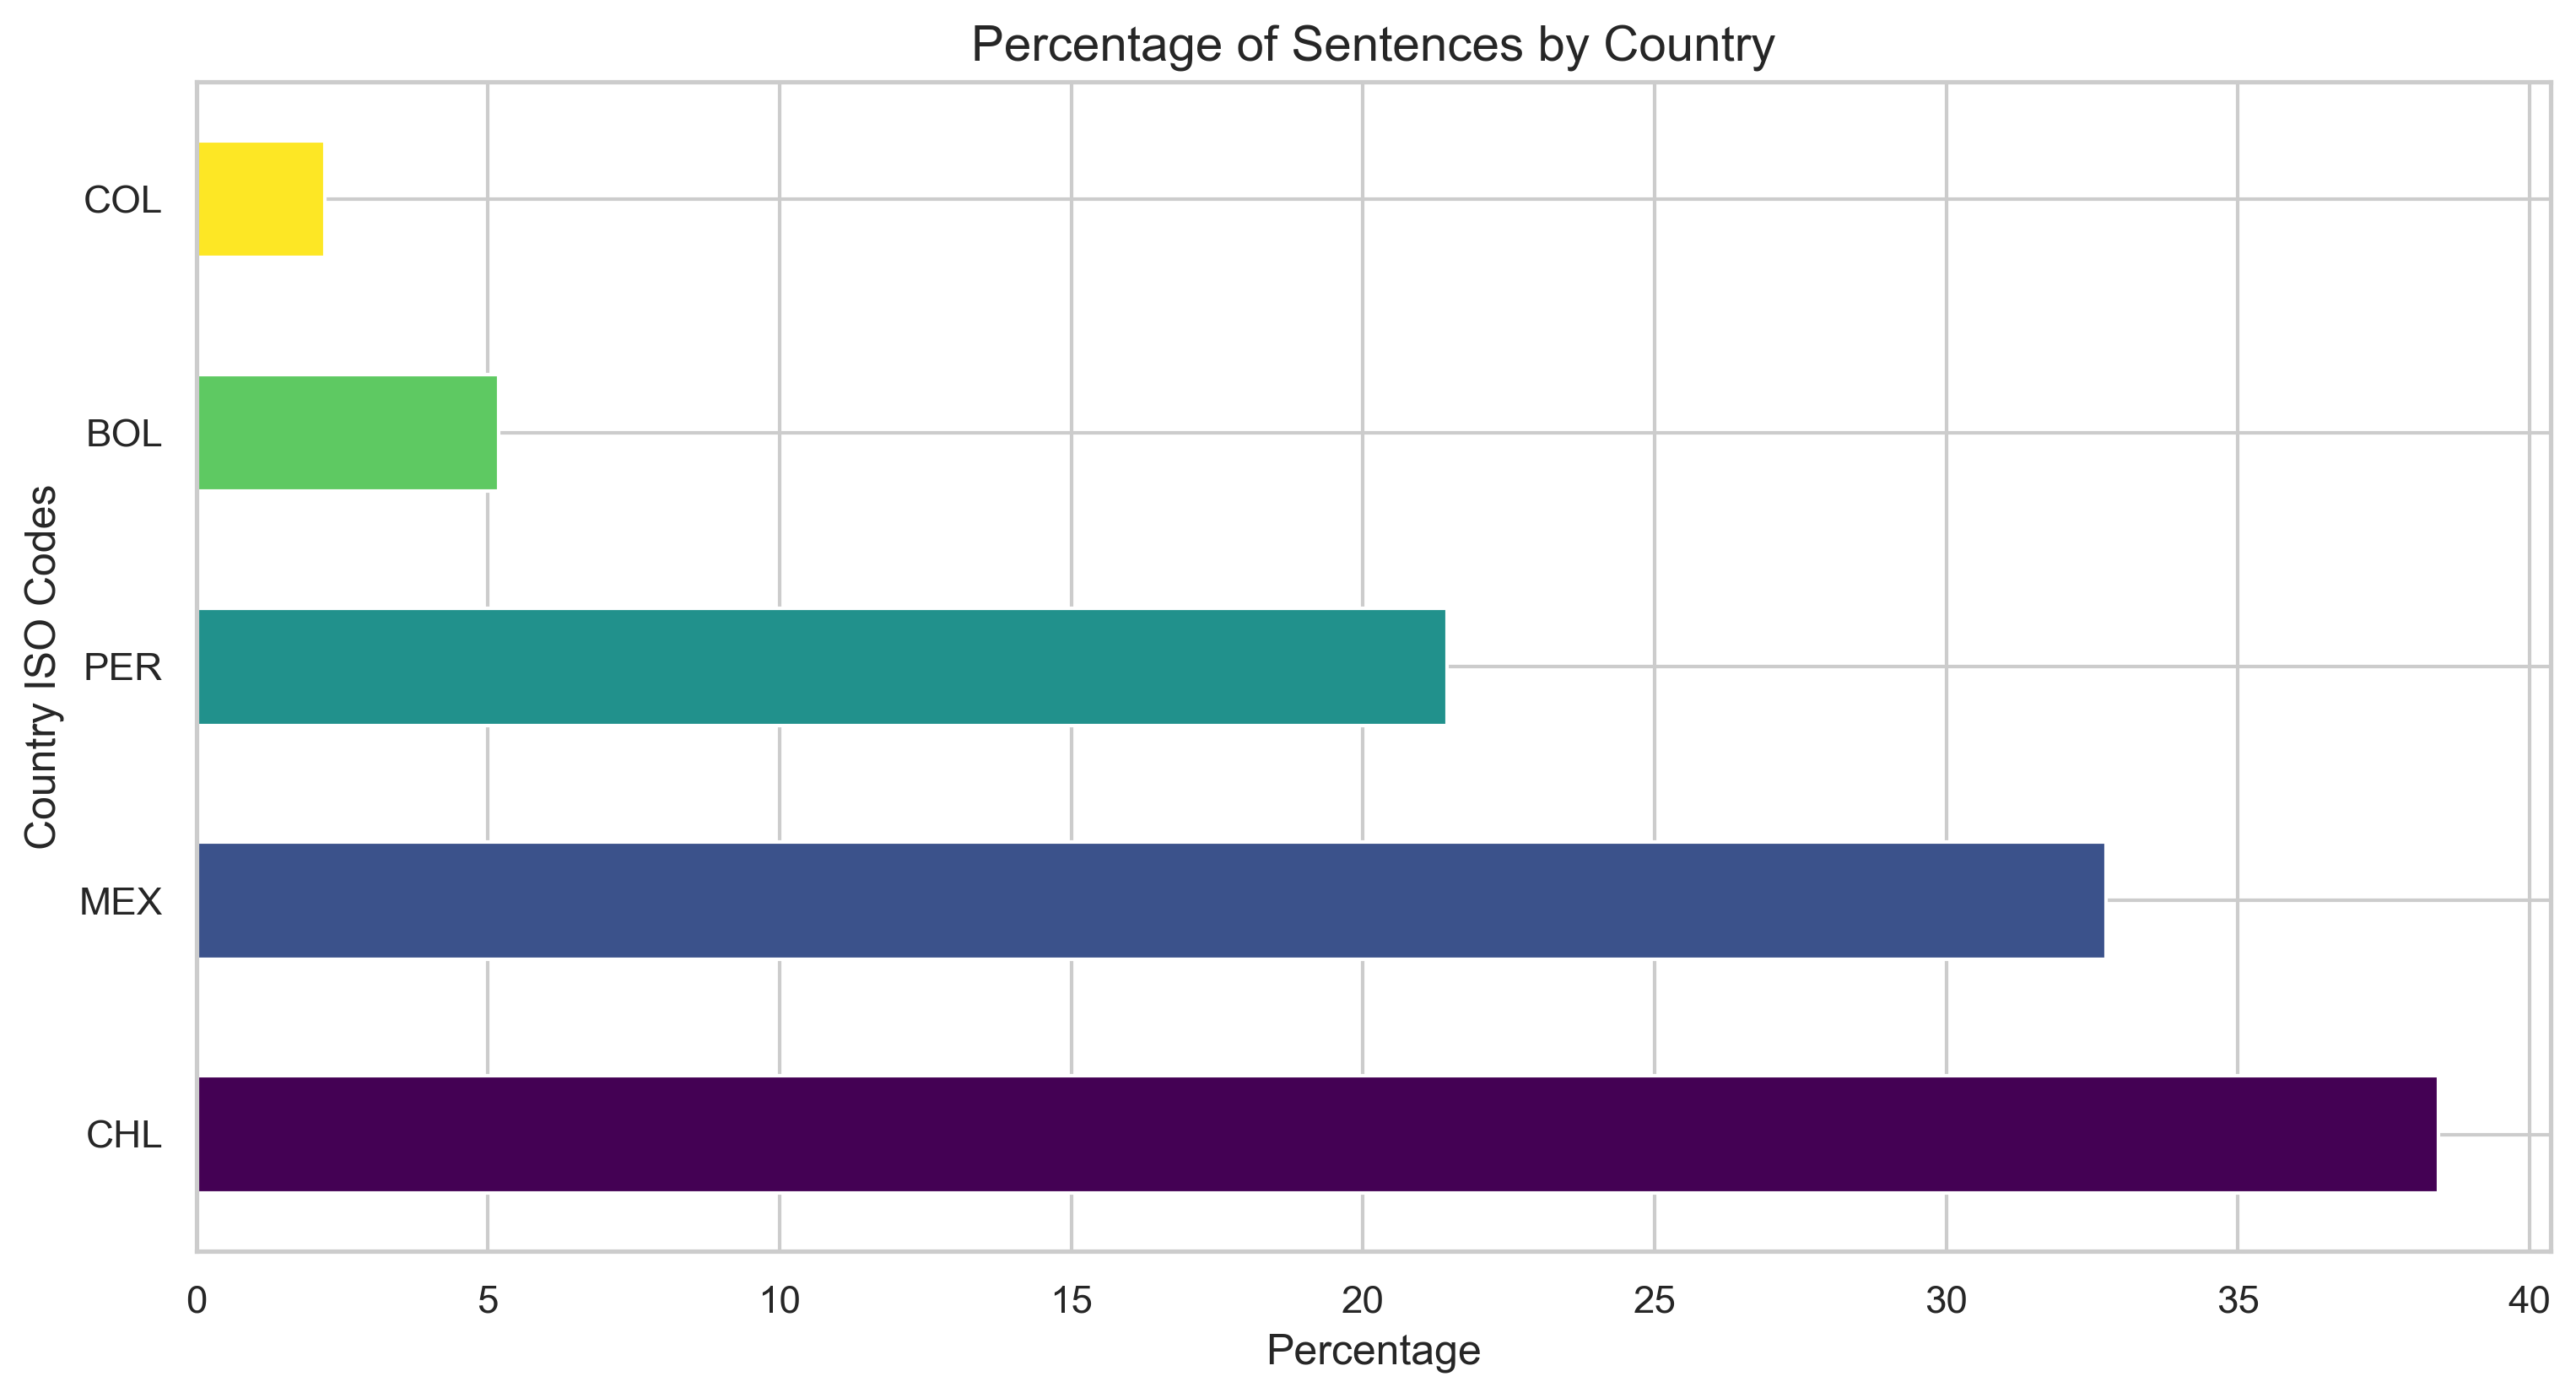
\includegraphics[width=0.8\textwidth]{/Users/sarabcidf/Desktop/ASDS/Dissertation/Python/country_percentage_distribution.png} 
\end{figure}

\begin{figure}[h]
	\centering
	\caption{Populist and non-populist balance}
	\label{fig:yourfigure}
	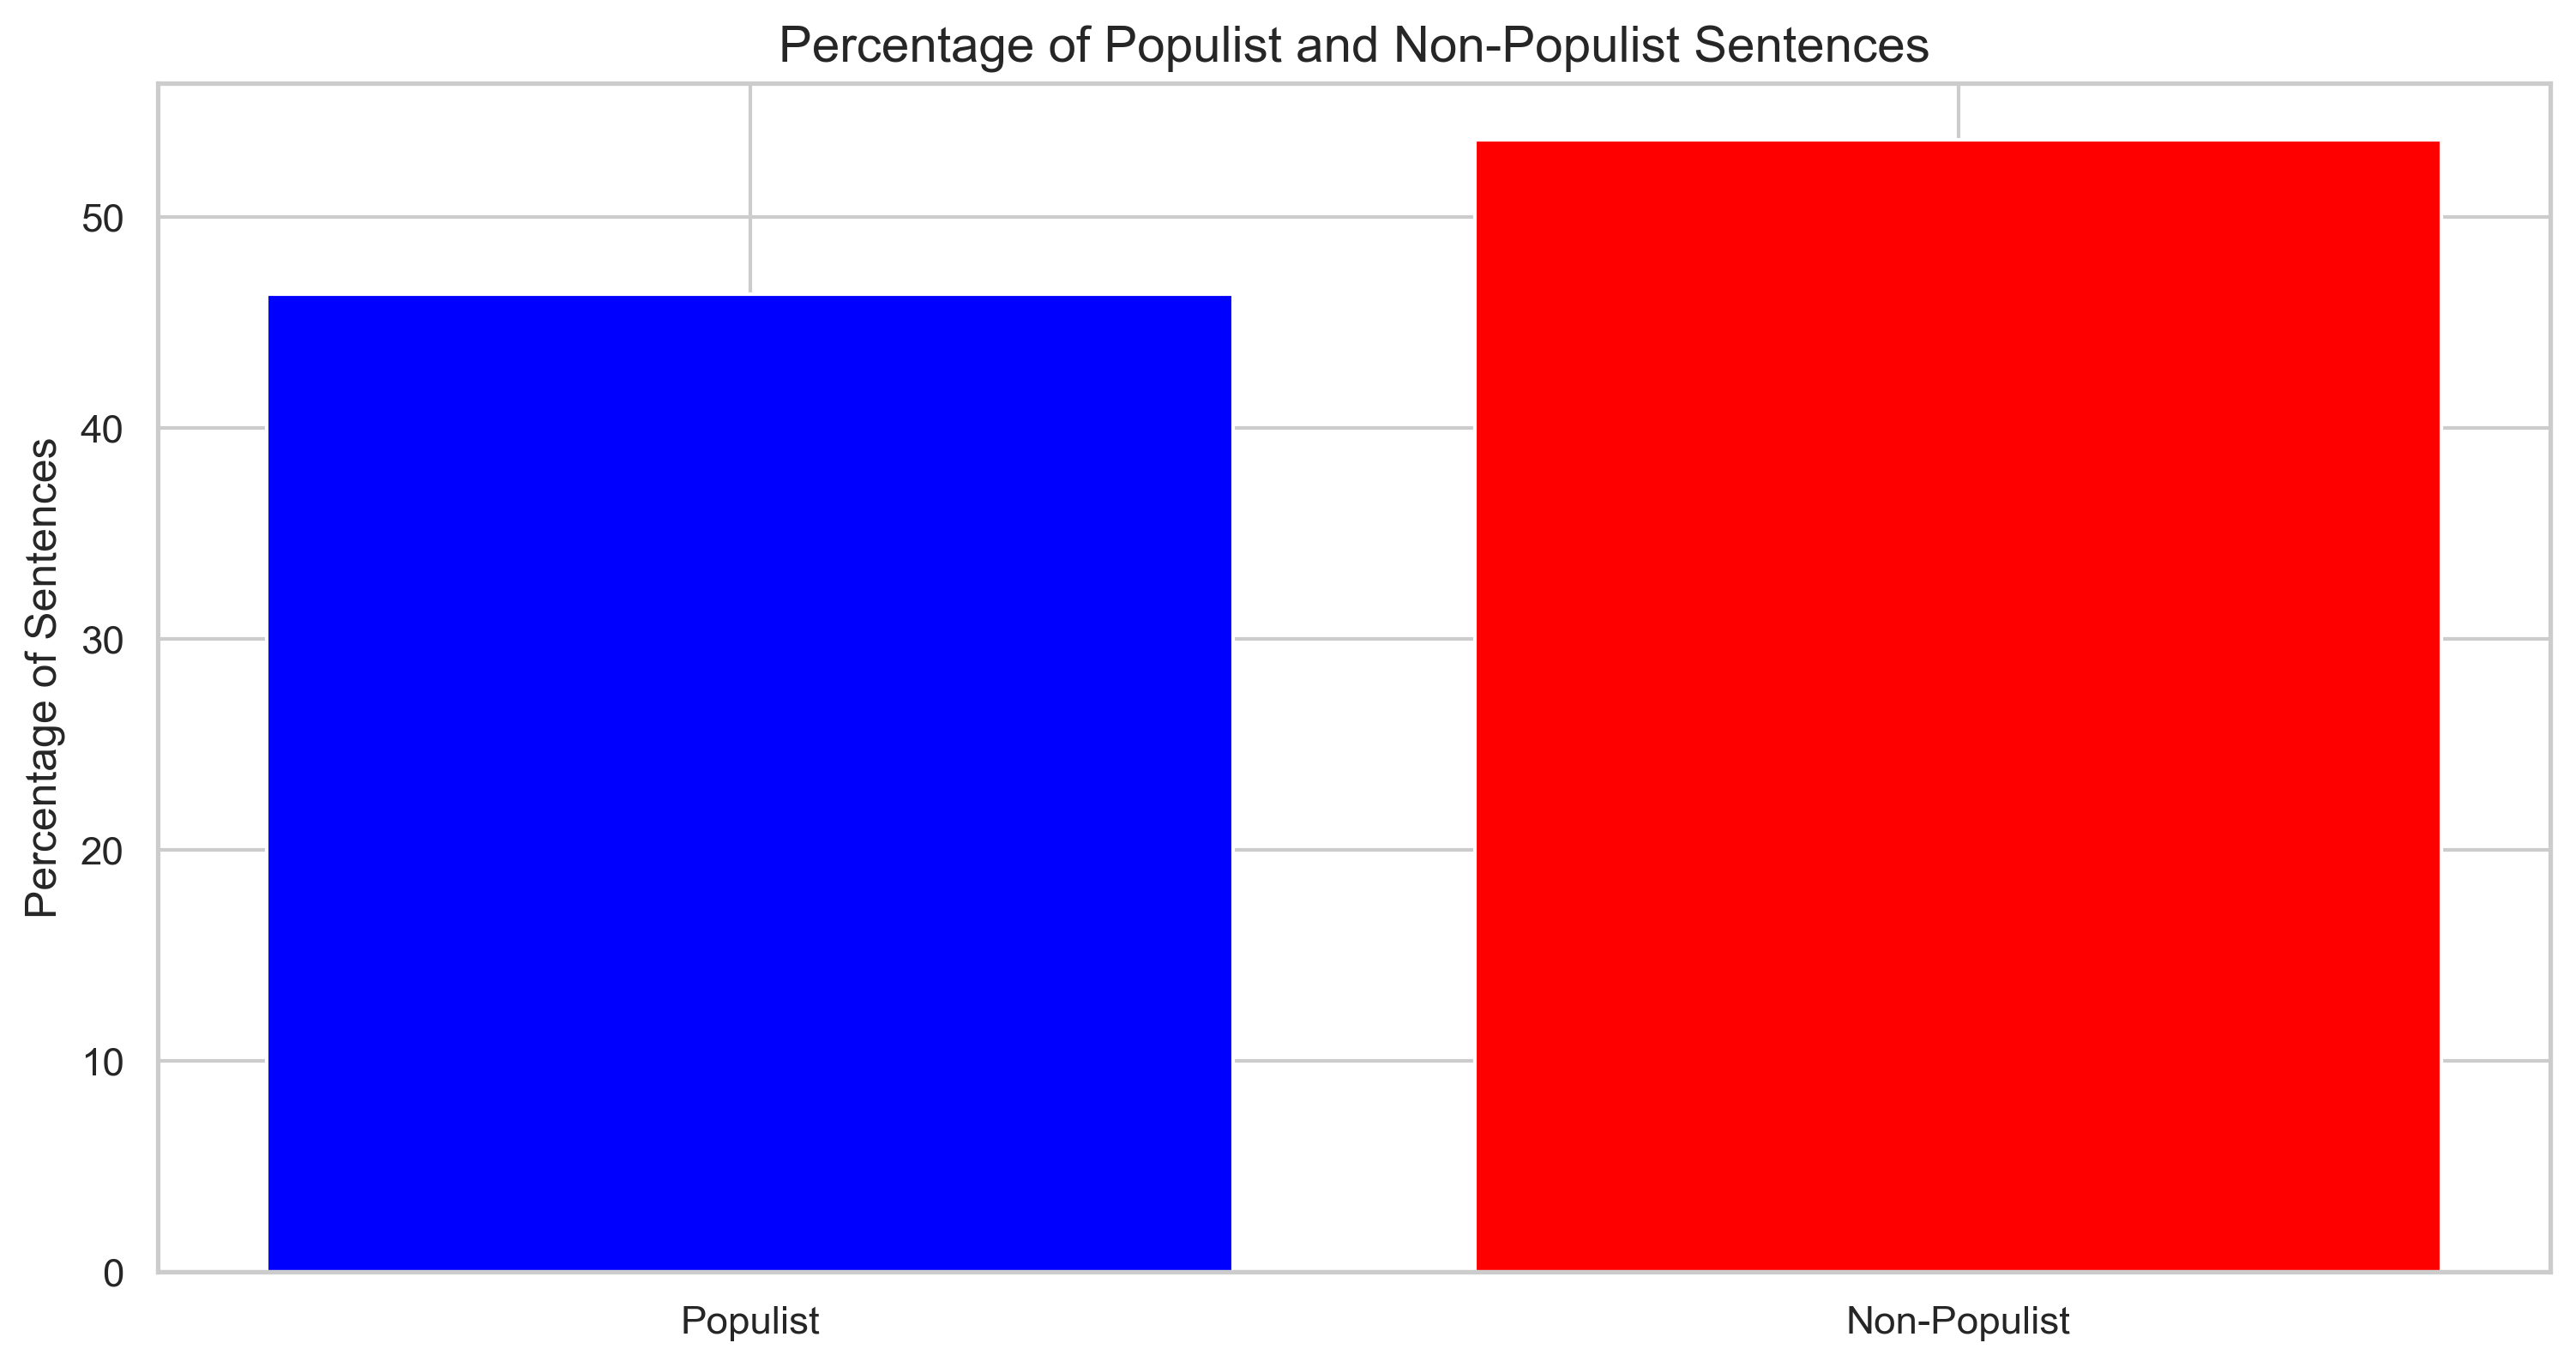
\includegraphics[width=0.8\textwidth]{/Users/sarabcidf/Desktop/ASDS/Dissertation/Python/populist_non_populist_percentage_distribution.png} 
\end{figure}

\begin{figure}[h]
	\centering
	\caption{Ideology balance}
	\label{fig:yourfigure}
	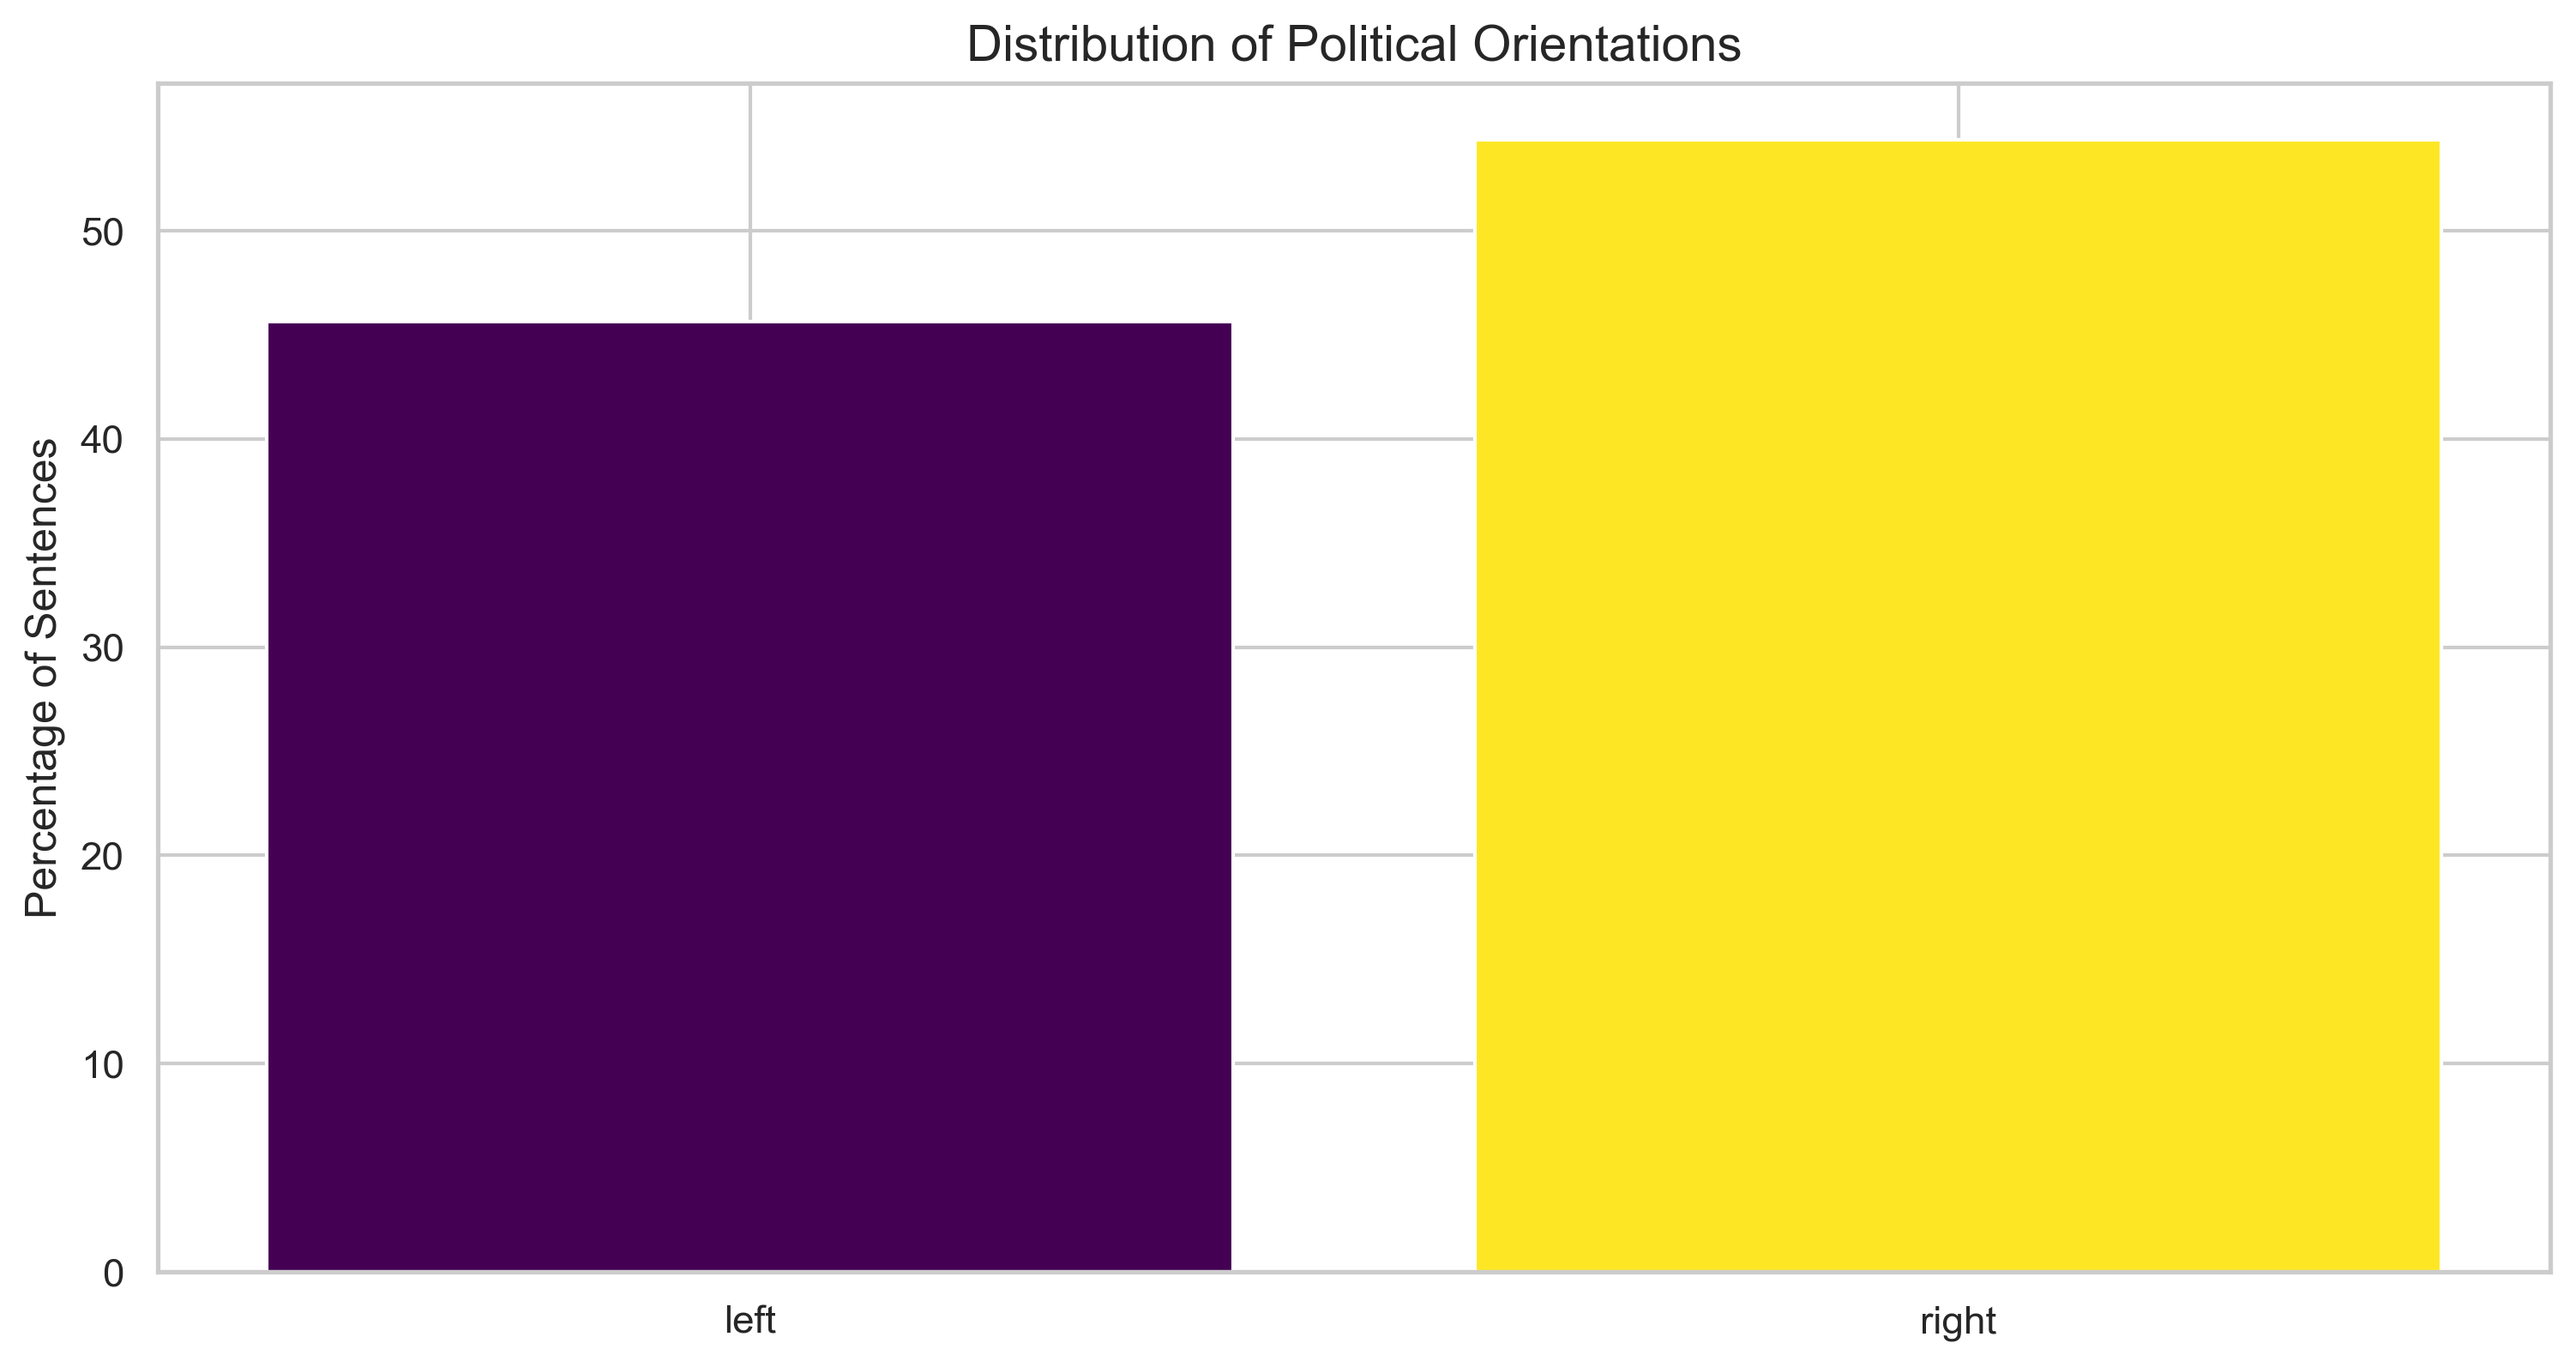
\includegraphics[width=0.8\textwidth]{/Users/sarabcidf/Desktop/ASDS/Dissertation/Python/political_orientations_percentage_distribution.png} 
\end{figure}

\section*{Results} 
\vspace{.25cm}

\noindent \textcolor{red}{I imagine I will first show performance metrics for the classifier/regressor. 
	Then I will show results of the application. I imagine some sort of graph or regression results for looking at the level of populism vs. the level of anti-elitism (however it is that I end up measuring the latter).} 

\section*{Discussion and Conclusions} 
\vspace{.25cm}

\noindent \textcolor{red}{Discussion and Conclusions here.}

\printbibliography

\noindent \textcolor{red}{The formatting of the references also needs work still!}

\end{document}
